\subsection{Разработка грида}
\label{sec:development:grid}

Грид выступает инструментом для отображения компонентов, перетянутых с палитры компонентов. Это основной компонент, занимающий большую часть экрана. Он представляет собой разметку с сеткой, размер которой может быть изменен.

\subsubsection{}Алгоритм Drag-n-drop
\

Создание и перемещение компонентов осуществляется методами, реализующими алгоритм Drag-n-drop. Для этого был разработан объект Movable, методы которого предоставлет методы $\$$dragCreate, $\$$dragPos и $\$$dragDestroy.

Метод $\$$dragCreate отвечает за начало перетягивания компонента. Библиотека Webix предполагает наличие метода с таким названием и выполнение им строго определенных функций, в частности, если начинает перетягиватся компонент, возвращать его DOM-элемент, иначе -- false.

Метод $\$$dragPos отвечает за перерисовку компонента и грида во время движения первого. 

Метод $\$$dragDestroy осуществляет финализацию процесса перетягивания компонента: очистку используемых ресурсов, убирание тени от движения компонента, вызов события окончания движения и т.д.

Все добавления компонентов записываются в историю изменений. На данный момент она поддерживает лишь откат добавления элементов, что в будущем будет доработано. Схема алгоритма разботы истории изменений представлена на рисунке~\ref{sec:dev:history}

\begin{figure}[ht]
  \centering
    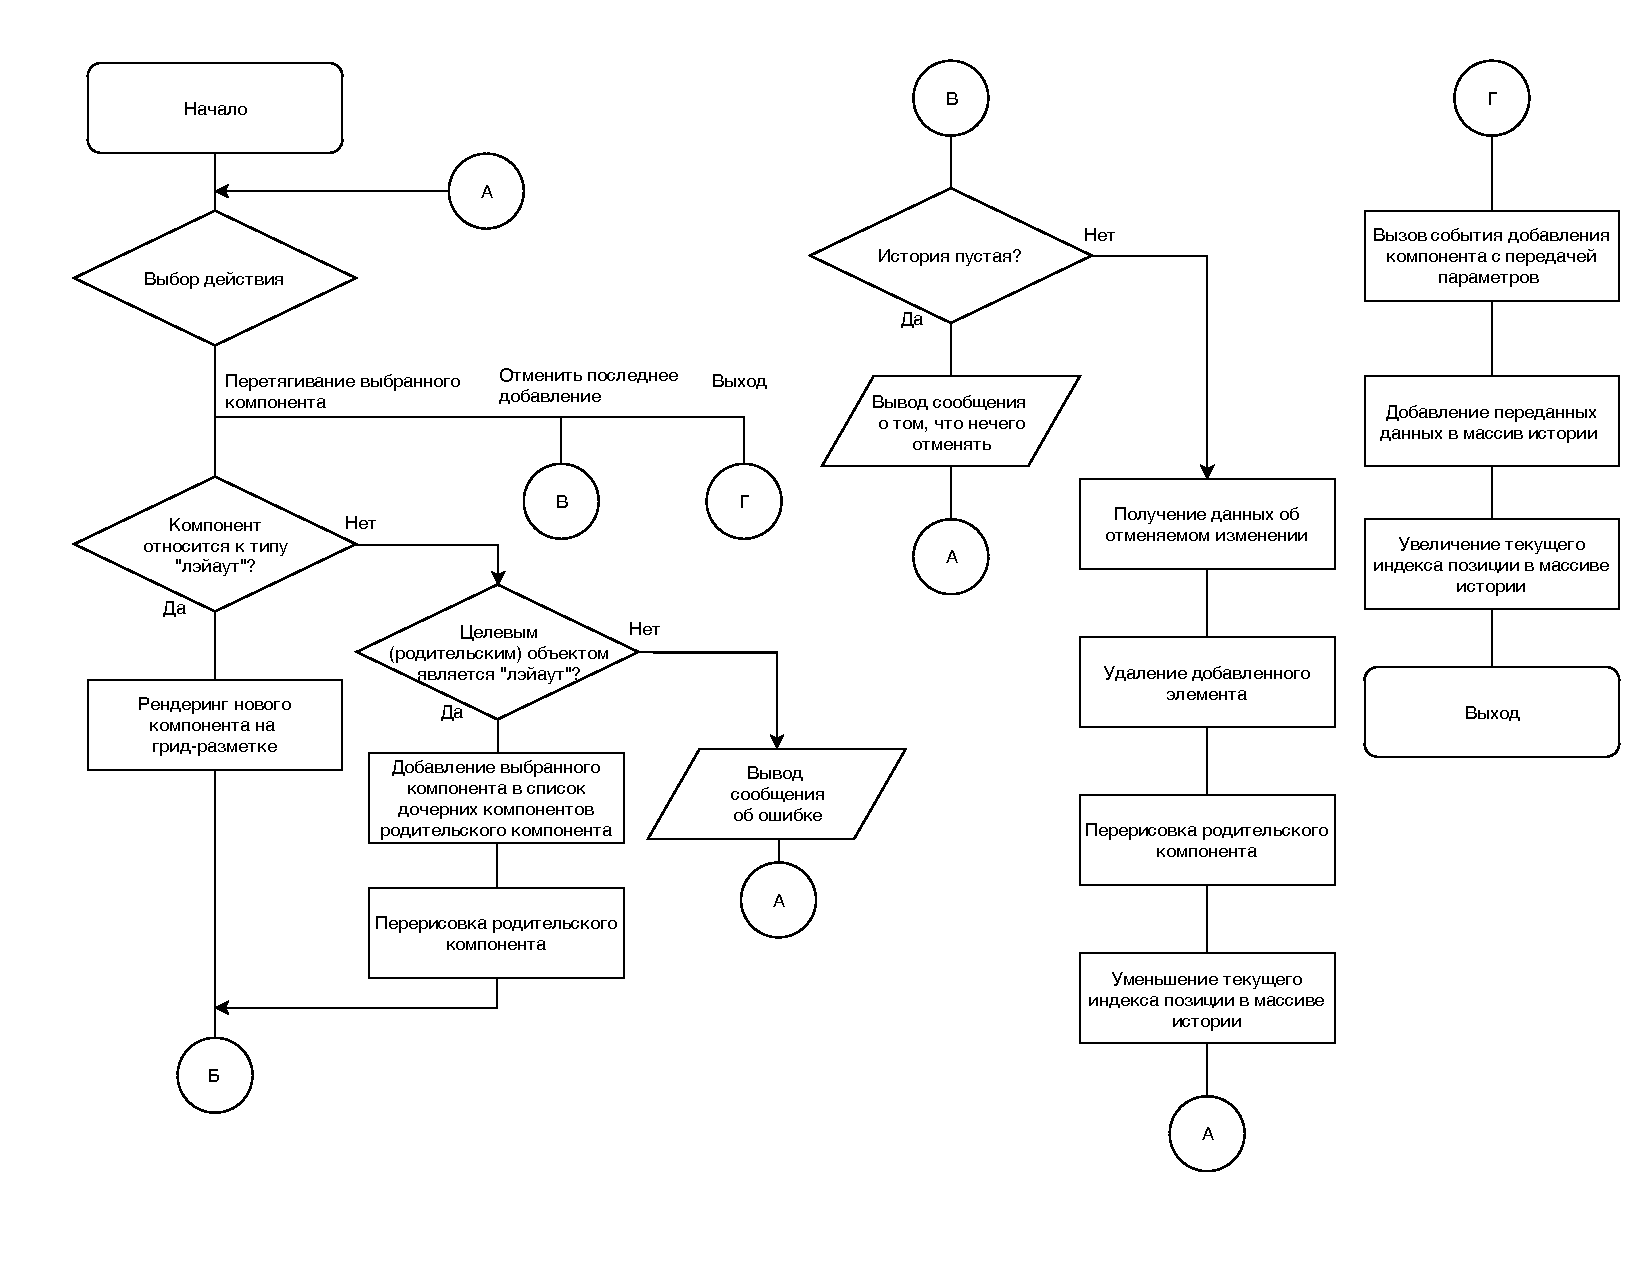
\includegraphics[scale=0.6]{schema_history.pdf}
    \caption{Алгоритм компоновки графических компонентов}
    \label{sec:dev:history}
\end{figure}

\subsubsection{}Разработка сетки грида и реализация <<магнитной привязки>>
\

Сетка грида выполняет не только декоративную функцию и несколько упрощает визуальное выравнивание компонентов, но и обладает свойством магнитной привязки.

Данный алгоритм предоставлет возможность редактировать размер сетки, суть которой заключается в том, что компоненты можно передвигать лишь с шагом, равным размеру клетки в пикселях. Вызовы метода stickToGrid выполняют дополнительные высчитывания координат места, куда будет позиционирован перетягиваемый компонент по окончании.

Также помимо сетки, присутствует тень от компонента, которая показывает, куда компонент будет помещен, когда пользователь отпустит нажатую для перетягивания компонента левую кнопку мыши или уберет палец от сенсорного экрана.

Алгоритм рисования тени предполагает вызов перерисовки тени на каждое событие движения мыши.

Добавление функицональности Drag-n-drop осуществляется путем вызова метода addDrop объекта DragControl, который доступен через глобальный объект webix.
Вызов метода происходит в методе инициализации грида $\$$init.

Добавление элемента на грид осуществляется методом внутренним приватным методом $\_$addMovableElement, который добавляет внутренние свойства к конфигу компонента, необходимые для дальнейшей работы.

Метод также добавляет необходимые обработчики событий как самому компоненту,так и всем его дочерним, что позволяет быть уверенным, что компоненты будут вести себя одинакого в разных сценариях использования.

Весь алгоритм компоновки в целом, а также некоторые его детали отображены на рисунке~\ref{sec:dev:composition}\pagebreak

\begin{figure}[ht]
  \centering
    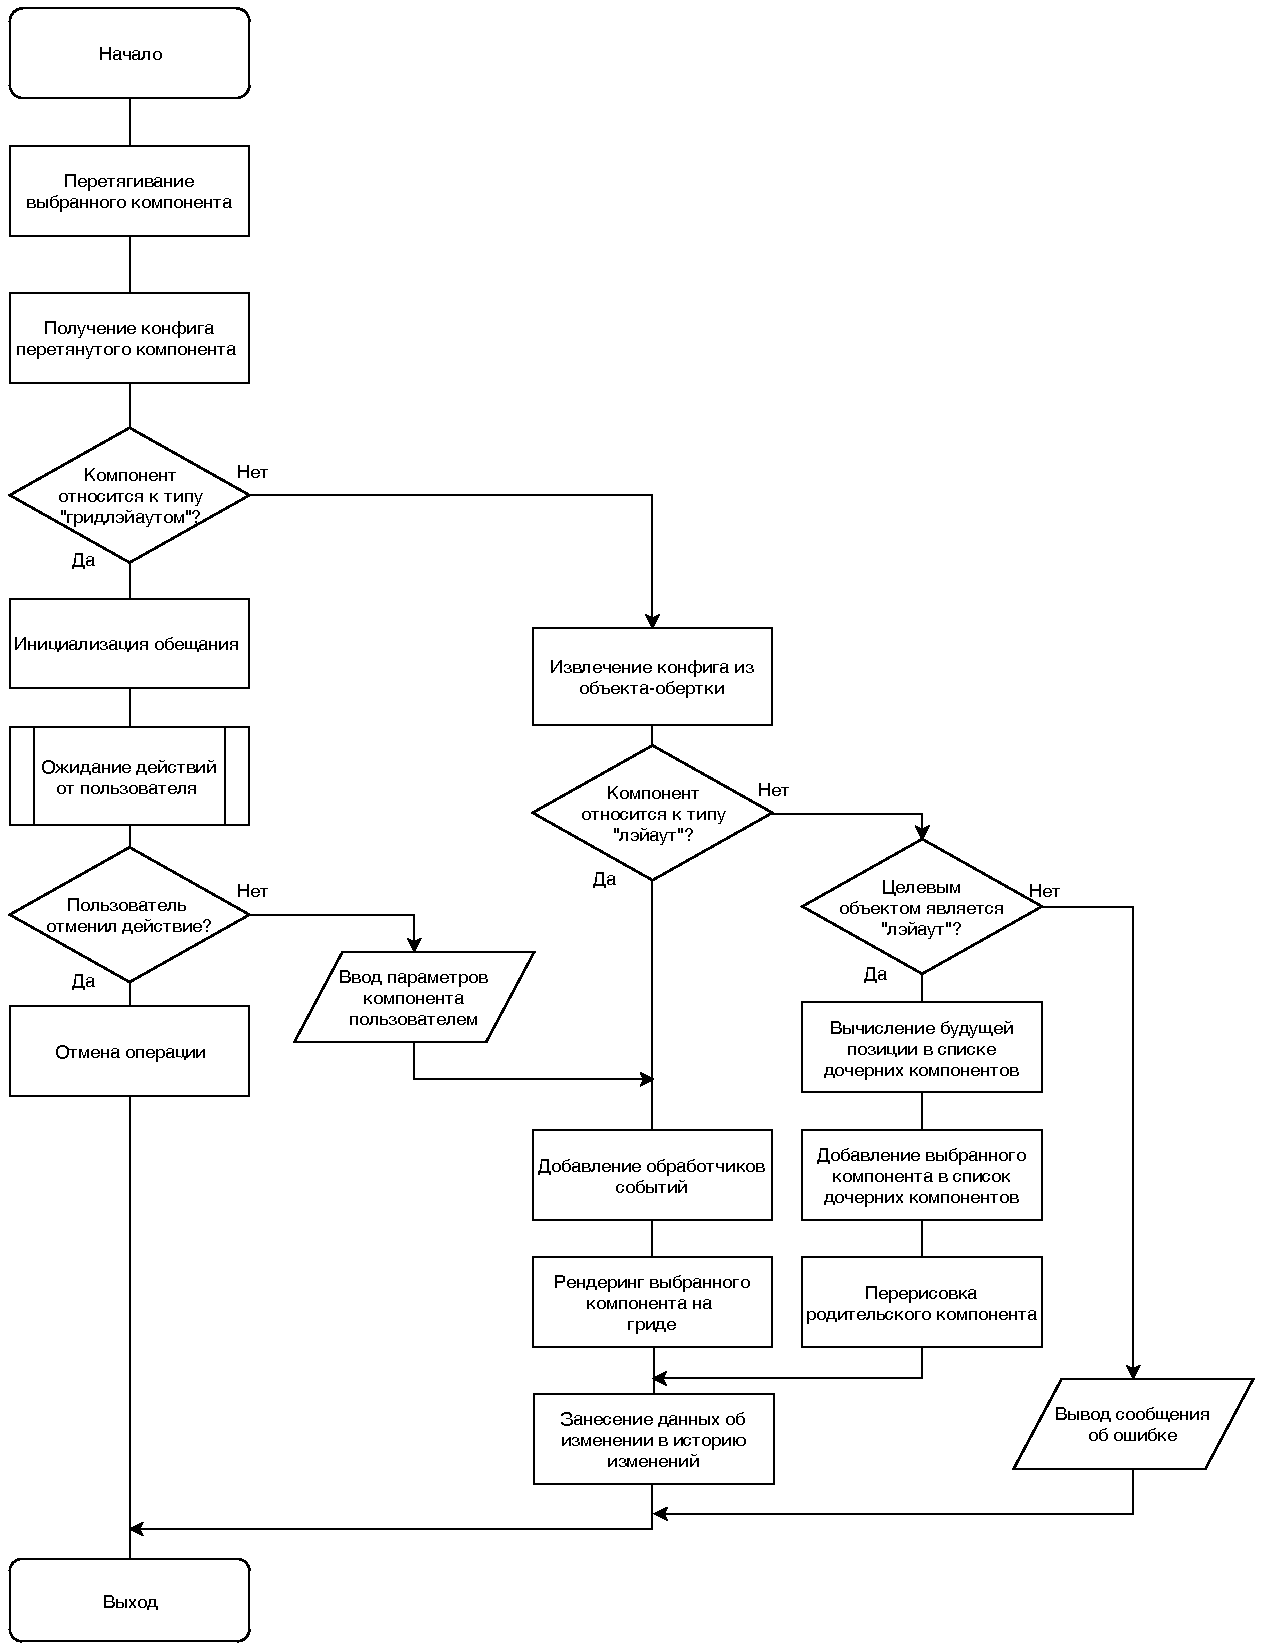
\includegraphics[scale=0.65]{schema_composition.pdf}
    \caption{Алгоритм компоновки графических компонентов}
    \label{sec:dev:composition}
\end{figure}